\documentclass[12pt,a4paper]{article}

% ─── Page Layout ───────────────────────────────────────────────────────────────
\usepackage[a4paper, margin=0.8in, headheight=14pt]{geometry}

% ─── Fonts (XeLaTeX) ───────────────────────────────────────────────────────────
\usepackage{fontspec}
\usepackage{unicode-math}
\setmainfont{TeX Gyre Pagella}
\setmonofont[Scale=0.88]{TeX Gyre Cursor}
\setmathfont{Latin Modern Math}

% ─── Packages ──────────────────────────────────────────────────────────────────
\usepackage{xcolor}
\usepackage{colortbl}
\usepackage{titlesec}
\usepackage{enumitem}
\usepackage{tabularx}
\usepackage{booktabs}
\usepackage{array}
\usepackage{amsmath}
\usepackage{tikz}
\usetikzlibrary{shapes.geometric, arrows.meta, positioning, calc, fit, decorations.pathreplacing}
\usepackage{tcolorbox}
\tcbuselibrary{skins, breakable}
\usepackage{hyperref}
\usepackage{fancyhdr}
\usepackage{graphicx}
\usepackage{microtype}
\hyphenpenalty=10000
\exhyphenpenalty=10000
\sloppy
\usepackage{caption}
\usepackage{setspace}
\usepackage{multirow}
\usepackage{tocloft}

% ─── Q&A helper ────────────────────────────────────────────────────────────────
\newcommand{\Q}[1]{\textbf{#1}\par\noindent\ignorespaces}

% ─── Colour Palette ────────────────────────────────────────────────────────────
\definecolor{myred}{RGB}{196,30,58}
\definecolor{mydark}{RGB}{30,30,50}
\definecolor{mygreen}{RGB}{14,120,80}
\definecolor{myteal}{RGB}{0,130,140}
\definecolor{myamber}{RGB}{180,100,0}
\definecolor{mypurple}{RGB}{100,30,160}
\definecolor{mygray}{RGB}{246,247,249}
\definecolor{mgframe}{RGB}{180,185,200}
\definecolor{watermark}{RGB}{145,150,170}
\definecolor{hdrred}{RGB}{250,232,235}
\definecolor{hdrgreen}{RGB}{220,244,233}
\definecolor{hdrteal}{RGB}{220,242,244}
\definecolor{hdramber}{RGB}{253,242,215}
\definecolor{hdrpurple}{RGB}{238,228,255}
\definecolor{hdrgray}{RGB}{238,240,245}
\definecolor{rowalt}{RGB}{250,251,253}

% ─── Section Formatting ────────────────────────────────────────────────────────
\titleformat{\section}
  {\large\bfseries\color{myred}}{\thesection.}{0.5em}{}
  [\vspace{1pt}{\color{myred}\rule{\linewidth}{0.8pt}}]
\titleformat{\subsection}
  {\normalsize\bfseries\color{myteal}}{\thesubsection}{0.5em}{}
\titlespacing*{\section}{0pt}{18pt}{7pt}
\titlespacing*{\subsection}{0pt}{11pt}{4pt}

% ─── Paragraph ─────────────────────────────────────────────────────────────────
\setlength{\parindent}{0pt}
\setlength{\parskip}{4pt}

% ─── TOC Styling ───────────────────────────────────────────────────────────────
\renewcommand{\cfttoctitlefont}{\large\bfseries\color{myred}}
\renewcommand{\cftaftertoctitle}{\par\noindent{\color{myred}\rule{\linewidth}{0.8pt}}}
\setlength{\cftbeforetoctitleskip}{0pt}
\setlength{\cftaftertoctitleskip}{6pt}
\renewcommand{\cftsecfont}{\normalsize\bfseries\color{mydark}}
\renewcommand{\cftsecpagefont}{\normalsize\bfseries\color{mydark}}
\renewcommand{\cftsecleader}{\cftdotfill{\cftdotsep}}
\setlength{\cftbeforesecskip}{7pt}
\renewcommand{\cftsubsecfont}{\small\color{mydark}}
\renewcommand{\cftsubsecpagefont}{\small\color{mydark}}
\setlength{\cftbeforesubsecskip}{3pt}
\setlength{\cftsubsecindent}{1.4em}

% ─── Table helpers ─────────────────────────────────────────────────────────────
\renewcommand{\arraystretch}{1.45}
\setlength{\tabcolsep}{6pt}
\arrayrulecolor{mydark}
\newcolumntype{B}[1]{>{\small\bfseries\raggedright\arraybackslash}m{#1}}
\newcolumntype{Y}{>{\small\raggedright\arraybackslash}X}
\renewcommand{\tabularxcolumn}[1]{m{#1}}

% ─── Header / Footer ───────────────────────────────────────────────────────────
\pagestyle{fancy}
\fancyhf{}
\fancyhead[L]{\small\color{myred}\textbf{PE-EC701C}\;\color{mydark}--- Mobile Communication and Networks}
\fancyhead[R]{\small\color{myteal}\textbf{Module 2 Notes}}
\fancyfoot[C]{\small\color{mydark}\thepage}
\fancyfoot[R]{\small\color{watermark}\textit{\copyright\ Biraj}}
\renewcommand{\headrulewidth}{0.5pt}
\renewcommand{\footrulewidth}{0.3pt}

% ─── Hyperref ──────────────────────────────────────────────────────────────────
\hypersetup{
  colorlinks=true, linkcolor=myteal, urlcolor=myteal,
  pdfauthor={Biraj Sarkar},
  pdftitle={PE-EC701C --- Module 2 Notes}
}

% ─── tcolorbox styles ──────────────────────────────────────────────────────────
\tcbset{
  tikzbox/.style={
    colback=mygray, colframe=mgframe, boxrule=0.6pt, arc=4pt,
    left=8pt, right=8pt, top=6pt, bottom=6pt,
    colbacktitle=mgframe, coltitle=mydark,
    fonttitle=\small\bfseries
  },
  defbox/.style={
    colback=hdrgreen, colframe=mygreen, boxrule=0.8pt, arc=4pt,
    left=9pt, right=9pt, top=6pt, bottom=6pt,
    colbacktitle=mygreen, coltitle=white,
    fonttitle=\small\bfseries
  },
  formulabox/.style={
    colback=hdrteal, colframe=myteal, boxrule=0.8pt, arc=4pt,
    left=9pt, right=9pt, top=7pt, bottom=7pt,
    colbacktitle=myteal, coltitle=white,
    fonttitle=\small\bfseries
  },
  examplebox/.style={
    colback=hdramber, colframe=myamber, boxrule=0.8pt, arc=4pt,
    left=9pt, right=9pt, top=6pt, bottom=6pt,
    colbacktitle=myamber, coltitle=white,
    fonttitle=\small\bfseries
  },
  masonbox/.style={
    colback=hdrpurple, colframe=mypurple, boxrule=0.8pt, arc=4pt,
    left=9pt, right=9pt, top=6pt, bottom=6pt,
    colbacktitle=mypurple, coltitle=white,
    fonttitle=\small\bfseries
  },
  exambox/.style={
    colback=hdrpurple, colframe=mypurple, boxrule=1pt, arc=5pt,
    left=10pt, right=10pt, top=8pt, bottom=8pt,
    colbacktitle=mypurple, coltitle=white,
    fonttitle=\bfseries,
    breakable, title after break={\textbf{Frequently Asked / Viva Questions (contd.)}}}
}
\tcbset{breakable}

% ─── TikZ styles ───────────────────────────────────────────────────────────────
\tikzset{
  block/.style={rectangle, draw=myteal, fill=hdrteal,
    text width=2.4cm, align=center, minimum height=0.95cm,
    font=\small, rounded corners=3pt, line width=0.7pt},
  redblock/.style={rectangle, draw=myred, fill=hdrred,
    text width=2.4cm, align=center, minimum height=0.95cm,
    font=\small, rounded corners=3pt, line width=0.7pt},
  netnode/.style={rectangle, draw=myteal, fill=hdrteal,
    text width=1.5cm, align=center, minimum height=0.8cm,
    font=\small, rounded corners=3pt, line width=0.7pt},
  sumjunc/.style={circle, draw=myamber, fill=hdramber,
    minimum size=0.62cm, font=\small, line width=0.8pt},
  snode/.style={circle, draw=mypurple, fill=hdrpurple,
    minimum size=0.55cm, font=\footnotesize, line width=0.7pt},
  arrow/.style={-Stealth, thick, color=mydark},
  redarrow/.style={-Stealth, thick, color=myred},
  line/.style={thick, color=mydark}
}

% ═══════════════════════════════════════════════════════════════════════════════
\begin{document}
% ═══════════════════════════════════════════════════════════════════════════════

\begin{center}
  {\LARGE\bfseries\color{myred} PE-EC701C --- Mobile Communication and Networks}\\[5pt]
  {\normalsize\color{mydark} Semester VII \quad$\bullet$\quad 3L:0T:0P \quad$\bullet$\quad 3 Credits}\\[3pt]
  {\normalsize\color{myteal}\textbf{Module 2 Exam Notes: Signal Propagation and Fading Channels}}\\[3pt]
  {\small\color{mydark} CGEC \;$|$\; B.Tech ECE (2023--27) \;$|$\; \textit{Biraj Sarkar}}
\end{center}
\noindent{\color{myred}\rule{\linewidth}{1.5pt}}
\vspace{2pt}

\hypersetup{linkcolor=mydark}
\tableofcontents
\hypersetup{linkcolor=myteal}
\newpage

% ===============================================================================
\section{Radio Wave Propagation Mechanisms}
% ===============================================================================

Radio signal propagation in mobile networks is highly dynamic. As electromagnetic waves travel from the transmitter (TX) to the receiver (RX), they interact with physical structures in the environment. These interactions are categorized into three basic mechanisms:

\begin{tcolorbox}[defbox]
\textbf{Basic Propagation Mechanisms:}
\begin{itemize}[leftmargin=*, itemsep=3pt, topsep=0pt]
  \item \textbf{Reflection:} Occurs when a wave impinges upon an object with very large dimensions compared to the wavelength ($\lambda$) (e.g., the surface of the earth, large buildings).
  \item \textbf{Diffraction (Knife-Edge):} Occurs when the radio path between the TX and RX is obstructed by an impenetrable body with sharp edges (e.g., hills, roofs), bending the wave around the obstacle.
  \item \textbf{Scattering:} Occurs when the medium contains objects with dimensions smaller than the wavelength ($\lambda$) and where the number of obstacles per unit volume is large (e.g., foliage, street signs).
\end{itemize}
\end{tcolorbox}

\begin{tcolorbox}[tikzbox, title={Physical Representation of Propagation Mechanisms}]
\centering
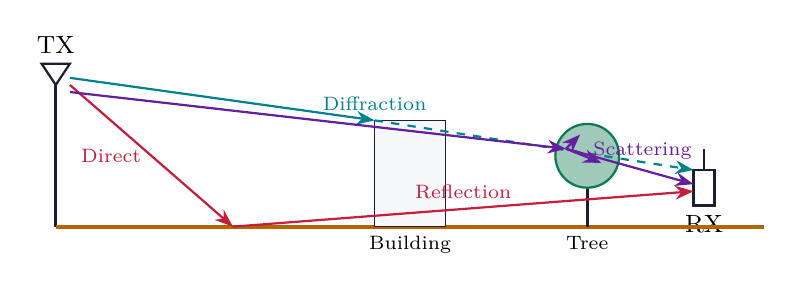
\begin{tikzpicture}[scale=0.9]
  % Transmitter tower
  \draw[line, line width=1.2pt] (0,0) -- (0,2);
  \draw[line] (0,2) -- (-0.2, 2.3) -- (0.2, 2.3) -- cycle;
  \node[above] at (0,2.3) {\small TX};

  % Receiver (Mobile)
  \draw[line, line width=1pt] (9,0.3) rectangle (9.3, 0.8);
  \draw[line] (9.15, 0.8) -- (9.15, 1.1);
  \node[below] at (9.15,0.3) {\small RX};

  % Obstacles
  % Large ground plane for reflection
  \draw[line, line width=1.5pt, color=myamber] (0,0) -- (10,0);
  
  % A sharp obstacle (building/wall) for diffraction
  \fill[draw=mydark, fill=mygray] (4.5,0) rectangle (5.5,1.5);
  \node[below, font=\scriptsize] at (5,0) {Building};

  % Scattering element (foliage/tree)
  \draw[line, line width=1pt] (7.5,0) -- (7.5,0.7);
  \draw[fill=mygreen!40, draw=mygreen, thick] (7.5,1.0) circle (0.45cm);
  \node[below, font=\scriptsize] at (7.5,0) {Tree};

  % Reflection Path
  \draw[arrow, color=myred] (0.2, 2.0) -- (2.5, 0) node[midway, left, font=\scriptsize] {Direct};
  \draw[arrow, color=myred] (2.5, 0) -- (9.0, 0.5) node[pos=0.5, above, font=\scriptsize] {Reflection};

  % Diffraction Path
  \draw[arrow, color=myteal] (0.2, 2.1) -- (4.5, 1.5);
  \draw[arrow, color=myteal, dashed] (4.5, 1.5) -- (9.0, 0.8);
  \node[above, font=\scriptsize, color=myteal] at (4.5,1.5) {Diffraction};

  % Scattering Path
  \draw[arrow, color=mypurple] (0.2, 1.9) -- (7.2, 1.1);
  \draw[arrow, color=mypurple] (7.2, 1.1) -- (7.4, 1.3);
  \draw[arrow, color=mypurple] (7.2, 1.1) -- (7.7, 0.9);
  \draw[arrow, color=mypurple] (7.2, 1.1) -- (9.0, 0.6) node[pos=0.6, above, font=\scriptsize] {Scattering};
\end{tikzpicture}
\end{tcolorbox}

% ===============================================================================
\section{Large-Scale Signal Propagation and Shadowing}
% ===============================================================================

\subsection{Path Loss and Log-Normal Shadowing}
Large-scale propagation models predict the average received signal strength over large TX-RX separation distances (hundreds or thousands of meters).
\begin{itemize}[leftmargin=*, itemsep=3.0pt]
  \item \textbf{Path Loss ($P_L$):} The attenuation of signal power as it propagates through space, modeled by:
    \begin{equation}
      P_L(d) \propto \left(\frac{d}{d_0}\right)^n
    \end{equation}
    Where $n$ is the path loss exponent and $d_0$ is a close-in reference distance.
  \item \textbf{Log-Normal Shadowing:} Represents slow fading caused by environmental obstructions (like buildings and trees) that block the line-of-sight. The received power exhibits random variations about the mean path loss, following a normal distribution when measured in decibels (dB).
\end{itemize}

\begin{tcolorbox}[formulabox, title={\textbf{Log-Normal Shadowing Model}}]
The overall path loss $P_L(d)$ in dB at distance $d$ is modeled as:
\begin{equation}
  P_L(d)[\text{dB}] = \overline{P_L}(d_0) + 10 n \log_{10}\left(\frac{d}{d_0}\right) + X_\sigma
\end{equation}
Where:
\begin{itemize}[leftmargin=*, itemsep=2pt, topsep=2pt]
  \item $\overline{P_L}(d_0) = 20\log_{10}\left(\frac{4\pi d_0}{\lambda}\right)$ is the free-space path loss at the reference distance $d_0$.
  \item $n$ is the path-loss exponent (typically 2 in free space, 3 to 5 in urban areas).
  \item $X_\sigma$ is a \textbf{zero-mean Gaussian random variable} (in dB) with standard deviation $\sigma$ (also in dB). It represents the shadowing variation.
\end{itemize}
\end{tcolorbox}

% ===============================================================================
\section{Small-Scale Fading and Multipath Parameters}
% ===============================================================================

Small-scale fading describes the rapid fluctuations of received signal amplitude and phase over very short travel distances (a few wavelengths) or short time durations.

\subsection{Multipath and Doppler Shift}
Multipath propagation occurs because the signal is reflected and scattered, arriving at the receiver via multiple paths with different amplitudes, phases, and delays.
\begin{itemize}[leftmargin=*, itemsep=3pt]
  \item \textbf{Doppler Shift ($f_d$):} The shift in received frequency due to the relative motion between the transmitter and mobile receiver:
    \begin{equation}
      f_d = \frac{v}{\lambda} \cos \theta = \frac{v \cdot f_c}{c} \cos \theta
    \end{equation}
    Where $v$ is the mobile velocity, $\lambda$ is the wavelength, $f_c$ is the carrier frequency, and $\theta$ is the arrival angle of the wave relative to the direction of motion.
\end{itemize}

\subsection{Multipath Channel Parameters}
To characterize a multipath channel, a \textbf{Power Delay Profile (PDP)} is measured by sending a short pulse and recording the received power levels at different delays ($\tau_i$).
\begin{tcolorbox}[formulabox, title={\textbf{Multipath Spread Metrics}}]
\begin{enumerate}[leftmargin=*, itemsep=4pt, label=\textbf{\arabic*.}]
  \item \textbf{Mean Excess Delay ($\overline{\tau}$):} The first moment of the power delay profile:
    \begin{equation}
      \overline{\tau} = \frac{\sum_i P(\tau_i) \tau_i}{\sum_i P(\tau_i)}
    \end{equation}
  \item \textbf{RMS Delay Spread ($\sigma_\tau$):} The square root of the second central moment of the PDP:
    \begin{equation}
      \sigma_\tau = \sqrt{\overline{\tau^2} - (\overline{\tau})^2} \quad \text{where } \overline{\tau^2} = \frac{\sum_i P(\tau_i) \tau_i^2}{\sum_i P(\tau_i)}
    \end{equation}
    \textbf{Significance:} Measures the multipath time dispersion.
  \item \textbf{Coherence Bandwidth ($B_c$):} The frequency range over which the channel passes all spectral components with equal gain and linear phase:
    \begin{equation}
      B_c \approx \frac{1}{50\sigma_\tau} \quad (\text{for } 0.9 \text{ frequency correlation}), \quad B_c \approx \frac{1}{5\sigma_\tau} \quad (\text{for } 0.5 \text{ frequency correlation})
    \end{equation}
\end{enumerate}
\end{tcolorbox}

\begin{tcolorbox}[tikzbox, title={Multipath Power Delay Profile (PDP)}]
\centering
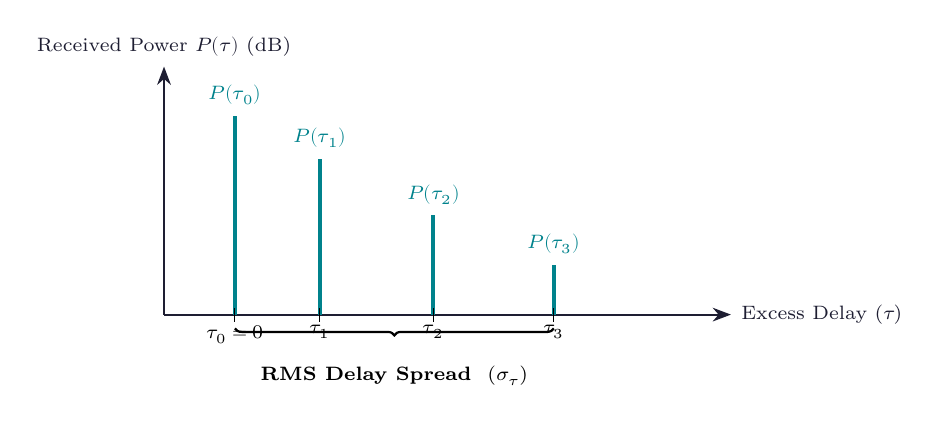
\begin{tikzpicture}[scale=0.9, every node/.style={font=\scriptsize}]
  \draw[arrow] (0,0) -- (8,0) node[right] {Excess Delay ($\tau$)};
  \draw[arrow] (0,0) -- (0,3.5) node[above] {Received Power $P(\tau)$ (dB)};

  % Multi-path spikes
  \draw[line width=1.5pt, color=myteal] (1,0) -- (1,2.8) node[above] {$P(\tau_0)$};
  \draw[line width=1.5pt, color=myteal] (2.2,0) -- (2.2,2.2) node[above] {$P(\tau_1)$};
  \draw[line width=1.5pt, color=myteal] (3.8,0) -- (3.8,1.4) node[above] {$P(\tau_2)$};
  \draw[line width=1.5pt, color=myteal] (5.5,0) -- (5.5,0.7) node[above] {$P(\tau_3)$};

  \draw (1,-0.1) -- (1,0.1) node[below=3pt] {$\tau_0=0$};
  \draw (2.2,-0.1) -- (2.2,0.1) node[below=3pt] {$\tau_1$};
  \draw (3.8,-0.1) -- (3.8,0.1) node[below=3pt] {$\tau_2$};
  \draw (5.5,-0.1) -- (5.5,0.1) node[below=3pt] {$\tau_3$};

  % Label showing delay spread
  \draw[thick, decoration={brace, mirror, raise=5pt}, decorate] (1,0) -- (5.5,0);
  \node[below=15pt] at (3.25,0) {\textbf{RMS Delay Spread } ($\sigma_\tau$)};
\end{tikzpicture}
\end{tcolorbox}

\subsection{Doppler Spread and Coherence Time}
While delay spread characterizes the time-dispersive nature of the channel, Doppler spread characterizes its time-varying nature:
\begin{itemize}[leftmargin=*, itemsep=3.0pt]
  \item \textbf{Doppler Spread ($B_D$):} The range of frequencies over which the received Doppler spectrum is non-zero. It equals the maximum Doppler shift $f_m = v/\lambda$.
  \item \textbf{Coherence Time ($T_c$):} The time duration over which the channel impulse response remains virtually constant:
    \begin{equation}
      T_c \approx \frac{9}{16\pi f_m} \approx \frac{0.178}{f_m} \quad (\text{rigorous}), \quad T_c \approx \frac{0.423}{f_m} \quad (\text{standard approximation})
    \end{equation}
\end{itemize}

% ===============================================================================
\section{Fading Classification and Channel Models}
% ===============================================================================

\subsection{Fading Classification}
Small-scale fading is classified based on two independent mechanisms: time dispersion (delay spread vs. symbol period) and frequency dispersion (Doppler spread vs. symbol rate).

\begin{tcolorbox}[tikzbox, title={Small-Scale Fading Classification Hierarchy}]
\centering
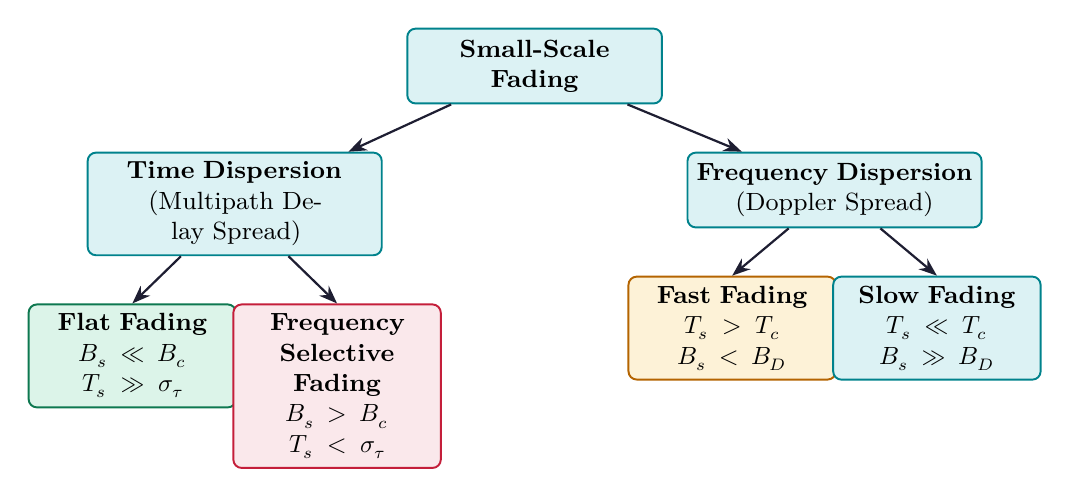
\begin{tikzpicture}[node distance=0.8cm and 0.8cm, every node/.style={font=\scriptsize}]
  \node[block, text width=3cm] (root) {\textbf{Small-Scale Fading}};
  
  \node[block, text width=3.5cm, below left=0.6cm and 0.3cm of root] (time) {\textbf{Time Dispersion}\\(Multipath Delay Spread)};
  \node[block, text width=3.5cm, below right=0.6cm and 0.3cm of root] (freq) {\textbf{Frequency Dispersion}\\(Doppler Spread)};

  \node[block, draw=mygreen, fill=hdrgreen, text width=2.4cm, below=0.6cm of time, xshift=-1.3cm] (flat) {\textbf{Flat Fading}\\$B_s \ll B_c$\\$T_s \gg \sigma_\tau$};
  \node[block, draw=myred, fill=hdrred, text width=2.4cm, below=0.6cm of time, xshift=1.3cm] (freqsel) {\textbf{Frequency\\Selective Fading}\\$B_s > B_c$\\$T_s < \sigma_\tau$};

  \node[block, draw=myamber, fill=hdramber, text width=2.4cm, below=0.6cm of freq, xshift=-1.3cm] (fast) {\textbf{Fast Fading}\\$T_s > T_c$\\$B_s < B_D$};
  \node[block, draw=myteal, fill=hdrteal, text width=2.4cm, below=0.6cm of freq, xshift=1.3cm] (slow) {\textbf{Slow Fading}\\$T_s \ll T_c$\\$B_s \gg B_D$};

  \draw[arrow] (root) -- (time);
  \draw[arrow] (root) -- (freq);
  \draw[arrow] (time) -- (flat.north);
  \draw[arrow] (time) -- (freqsel.north);
  \draw[arrow] (freq) -- (fast.north);
  \draw[arrow] (freq) -- (slow.north);
\end{tikzpicture}
\end{tcolorbox}

\subsection{Statistical Multipath Models}
When the received signal consists of multiple independent multipath waves, the envelope of the signal is modeled statistically:
\begin{enumerate}[label=\textbf{\arabic*.}, leftmargin=*, itemsep=4pt]
  \item \textbf{Rayleigh Fading (NLOS):} Used when there is no dominant line-of-sight (LOS) path. The received signal envelope $r$ is the sum of many independent scattered paths, following a Rayleigh probability density function (PDF):
    \begin{equation}
      p(r) = \frac{r}{\sigma^2} \exp\left(-\frac{r^2}{2\sigma^2}\right) \quad (r \ge 0)
    \end{equation}
    Where $\sigma^2$ is the time-average power of the received signal.
  \item \textbf{Ricean Fading (LOS):} Used when there is a dominant, direct line-of-sight (LOS) path in addition to multiple scattered paths. The envelope $r$ follows a Ricean PDF:
    \begin{equation}
      p(r) = \frac{r}{\sigma^2} \exp\left(-\frac{r^2 + A^2}{2\sigma^2}\right) I_0\left(\frac{A r}{\sigma^2}\right) \quad (r \ge 0)
    \end{equation}
    Where $A$ is the peak amplitude of the dominant LOS component, $\sigma^2$ is the variance of the scattered components, and $I_0(\cdot)$ is the modified Bessel function of the first kind of zeroth order.
  \item The channel is characterized by the \textbf{Ricean K-factor}:
    \begin{equation}
      K = \frac{\text{Power in dominant component}}{\text{Power in scattered components}} = \frac{A^2}{2\sigma^2}
    \end{equation}
    As $K \to 0$ ($-\infty$ dB), Ricean fading degenerates into Rayleigh fading. As $K \to \infty$, the channel becomes a static, fading-free LOS channel.
\end{enumerate}

\subsection{Level Crossing Rate (LCR) and Average Fade Duration (AFD)}
To design error correction codes and interleaver depths, we must know how often the signal falls below a threshold and how long it remains there:
\begin{itemize}[leftmargin=*, itemsep=3.5pt]
  \item \textbf{Level Crossing Rate (LCR, $N_R$):} The average number of times per second that the fading signal envelope crosses a specified threshold level $R$ in the positive direction:
    \begin{equation}
      N_R = \sqrt{2\pi} f_m \rho e^{-\rho^2}
    \end{equation}
    Where $f_m$ is the maximum Doppler shift and $\rho = R/R_{\text{rms}}$ is the normalized threshold level.
  \item \textbf{Average Fade Duration (AFD, $\overline{\tau}$):} The average period of time the received signal envelope remains below the threshold level $R$:
    \begin{equation}
      \overline{\tau} = \frac{e^{\rho^2} - 1}{\rho f_m \sqrt{2\pi}}
    \end{equation}
    \textbf{Significance:} AFD is inversely proportional to $f_m$. Fast-moving vehicles experience short fades, whereas slow-moving users experience long, deep fades.
\end{itemize}

% ===============================================================================
% MANDATORY QUICK REVISION PAGE
% ===============================================================================
\newpage
\begin{center}
  {\large\bfseries\color{myred} Quick Revision --- Module II}\\[3pt]
  {\small\color{mydark} Signal Propagation and Fading Channels $|$ PE-EC701C}
\end{center}
\noindent{\color{myred}\rule{\linewidth}{1.2pt}}
\vspace{4pt}

\begin{tcolorbox}[formulabox, title={\textbf{Key Formulas at a Glance}}]
\renewcommand{\arraystretch}{1.3}
\begin{tabularx}{\linewidth}{B{5.5cm} X}
Log-Normal Path Loss & $P_L(d)[\text{dB}] = \overline{P_L}(d_0) + 10 n \log_{10}(d/d_0) + X_\sigma$ \\
Doppler Shift & $f_d = \frac{v}{\lambda} \cos \theta$ \\
Mean Excess Delay & $\overline{\tau} = \frac{\sum P(\tau_i) \tau_i}{\sum P(\tau_i)}$ \\
RMS Delay Spread & $\sigma_\tau = \sqrt{\overline{\tau^2} - (\overline{\tau})^2}$ \\
Coherence Bandwidth ($0.9$ corr) & $B_c \approx \frac{1}{50\sigma_\tau}$ \\
Coherence Time & $T_c \approx \frac{0.423}{f_m}$ \quad ($f_m$ = max Doppler frequency) \\
Level Crossing Rate (LCR) & $N_R = \sqrt{2\pi} f_m \rho e^{-\rho^2}$ \\
Average Fade Duration (AFD) & $\overline{\tau} = \frac{e^{\rho^2} - 1}{\rho f_m \sqrt{2\pi}}$ \\
Ricean K-factor & $K = \frac{A^2}{2\sigma^2}$ \quad ($K \to 0$ for Rayleigh fading)
\end{tabularx}
\end{tcolorbox}

\begin{tcolorbox}[defbox, title={\textbf{One-Line Definitions}}]
\begin{itemize}[leftmargin=*, itemsep=2.5pt, topsep=0pt]
  \item \textbf{Lognormal Shadowing:} Slow fading caused by obstacles in the path, causing log-normal power variations.
  \item \textbf{Knife-Edge Diffraction:} Wave bending around sharp obstacles, modeled as an infinite half-plane.
  \item \textbf{Rayleigh Fading:} Statistical model for multi-path signal envelopes with no dominant line-of-sight path.
  \item \textbf{Ricean Fading:} Statistical model for multi-path envelopes containing a dominant line-of-sight component.
  \item \textbf{Coherence Bandwidth:} Range of frequencies over which the channel has constant gain and linear phase.
  \item \textbf{Coherence Time:} Maximum time separation over which two received signals are highly correlated in phase.
  \item \textbf{Flat Fading:} Fading where the channel bandwidth is larger than the signal bandwidth ($B_c \gg B_s$).
  \item \textbf{Frequency Selective Fading:} Fading where the signal bandwidth is wider than the channel coherence bandwidth ($B_s > B_c$).
\end{itemize}
\end{tcolorbox}

\begin{tcolorbox}[exambox, title={\textbf{Frequently Asked / Viva Questions}}]
\begin{enumerate}[topsep=0pt, label=\textbf{Q\arabic*.}, itemsep=5pt]
  \item \Q{Compare reflection, diffraction, and scattering.}
    Reflection occurs at objects much larger than the wavelength $\lambda$ (ground, walls). Diffraction occurs at sharp obstacles (hills, roofs) bending waves. Scattering occurs at objects smaller than $\lambda$ (leaves, rain).
  \item \Q{What causes small-scale fading in mobile channels?}
    It is caused by the interference of multiple reflected, diffracted, and scattered waves (multipath components) arriving at the receiver with arbitrary amplitudes and phases.
  \item \Q{What is the difference between flat and frequency selective fading? How are they classified?}
    Flat fading ($T_s \gg \sigma_\tau$ or $B_s \ll B_c$) preserves the pulse shape without ISI. Frequency selective fading ($T_s < \sigma_\tau$ or $B_s > B_c$) distorts the signal, causing Inter-Symbol Interference (ISI).
  \item \Q{What is the difference between slow and fast fading?}
    Fast fading ($T_s > T_c$) causes rapid channel changes within one symbol period, distorting the pulse envelope. Slow fading ($T_s \ll T_c$) keeps the channel constant over several symbols.
  \item \Q{Explain the physical significance of the K-factor in Ricean fading.}
    It represents the ratio of the power in the line-of-sight (LOS) direct path to the total power in the scattered paths. When $K=0$, it matches Rayleigh fading.
  \item \Q{How does vehicle velocity affect coherence time and average fade duration?}
    Higher velocity increases the Doppler shift ($f_m \propto v$). Since coherence time and AFD are inversely proportional to $f_m$, higher speeds shorten both.
  \item \Q{Why do we define a reference distance $d_0$ in path loss equations?}
    The close-in reference distance $d_0$ ensures the model operates in the far-field region of the transmitter antenna, where the power law approximation is valid.
  \item \Q{Describe the power delay profile (PDP) and its application.}
    A plot of received signal power as a function of excess time delay. It is used to compute mean excess delay, RMS delay spread, and coherence bandwidth.
  \item \Q{What is the significance of the level crossing rate (LCR)?}
    It helps determine the expected rate of fading occurrences below a threshold, which is critical for choosing interleaving depths and channel coding parameters.
  \item \Q{Explain the physical cause of a Doppler shift.}
    Relative movement between the mobile station and the base station changes the path length, resulting in a shift in received frequency.
  \item \Q{Under what condition does a Ricean distribution become a Rayleigh distribution?}
    When the direct line-of-sight component becomes completely blocked, its amplitude $A \to 0$. The K-factor becomes 0, and the Ricean distribution degrades to a Rayleigh distribution.
  \item \Q{Why does frequency selective fading cause Inter-Symbol Interference (ISI)?}
    Because the channel's delay spread $\sigma_\tau$ is larger than the symbol period $T_s$. This causes energy from a preceding symbol to leak into subsequent symbols.
\end{enumerate}
\tcbset{colbacktitle=myteal, coltitle=white}
\end{tcolorbox}

\begin{tcolorbox}[tikzbox, title={Fading Types Summary Table}]
\renewcommand{\arraystretch}{1.4}
\par\noindent
{\renewcommand{\arraystretch}{1.65}%
\begin{tabularx}{\linewidth}{|B{3.0cm}|Y|Y|}
\hline
\textbf{Fading Type} & \textbf{Relation} & \textbf{Primary Effect} \\
\hline
\textbf{Flat Fading} & $B_s \ll B_c$ \;/\; $T_s \gg \sigma_\tau$ & Amplitude fluctuates, pulse shape preserved. No ISI. \\[4pt]
\hline
\textbf{Freq. Selective} & $B_s > B_c$ \;/\; $T_s < \sigma_\tau$ & Signal distorted, severe ISI. Requires equalizer. \\[4pt]
\hline
\textbf{Fast Fading} & $T_s > T_c$ \;/\; $B_s < B_D$ & Channel changes within symbol. Distorts envelope. \\[4pt]
\hline
\textbf{Slow Fading} & $T_s \ll T_c$ \;/\; $B_s \gg B_D$ & Channel constant over many symbols. Normal detection. \\[4pt]
\hline
\end{tabularx}
}
\tcbset{colbacktitle=myteal, coltitle=white}
\end{tcolorbox}

\end{document}
